%==============================================================================
% Sjabloon poster bachproef
%==============================================================================
% Gebaseerd op document class `a0poster' door Gerlinde Kettl en Matthias Weiser
% Aangepast voor gebruik aan HOGENT door Jens Buysse en Bert Van Vreckem

\documentclass[a0,portrait]{hogent-poster}

% Info over de opleiding
\course{Bachelorproef}
\studyprogramme{toegepaste informatica}
\academicyear{2024-2025}
\institution{Hogeschool Gent, Valentin Vaerwyckweg 1, 9000 Gent}

% Info over de bachelorproef
\title{De invloed van geautomatiseerde spelers- en matchstatistieken bij volleybalclub Lindemans Aalst}
%\subtitle{Ondertitel (eventueel)}
\author{Youna Noynaert}
\email{youna.noynaert@student.hogent.be}
\supervisor{Lotte Van Steenberghe}
\cosupervisor{Joost Van Kerckhove (Lindemans Aalst)}

% Indien ingevuld, wordt deze informatie toegevoegd aan het einde van de
% abstract. Zet in commentaar als je dit niet wilt.
\specialisation{Systeem- en Netwerkbeheer}
\keywords{Lambda-calculus, Scheme}
\projectrepo{https://github.com/user/repo}

\begin{document}

\maketitle

\begin{abstract}
It's only a model.
You don't vote for kings. Who's that then? We found them. Ni! Ni! Ni! Ni!
The nose? On second thoughts, let's not go there. It is a silly place. Bloody Peasant! And the hat. She's a witch! Where'd you get the coconuts?
\end{abstract}

\begin{multicols}{2} % This is how many columns your poster will be broken into, a portrait poster is generally split into 2 columns

\section{Introductie}

Be quiet! Found them? In Mercia?! The coconut's tropical! But you are dressed as one… Well, what do you want? Knights of Ni, we are but simple travelers who seek the enchanter who lives beyond these woods.

Well, what do you want? It's only a model. Camelot! We found them. We shall say `Ni' again to you, if you do not appease us.

The nose? Shut up! Burn her! I am your king. You don't vote for kings.

You can't expect to wield supreme power just `cause some watery tart threw a sword at you! Well, we did do the nose. I don't want to talk to you no more, you empty-headed animal food trough water! I fart in your general direction! Your mother was a hamster and your father smelt of elderberries! Now leave before I am forced to taunt you a second time!

Why do you think that she is a witch? We want a shrubbery!! I don't want to talk to you no more, you empty-headed animal food trough water! I fart in your general direction! Your mother was a hamster and your father smelt of elderberries! Now leave before I am forced to taunt you a second time!

\section{Experimenten}

A newt? Camelot! Why? No, no, no! Yes, yes. A bit. But she's got a wart.

Shut up! I dunno. Must be a king. Who's that then? Look, my liege! On second thoughts, let's not go there. It is a silly place.

Shut up! Will you shut up?! No, no, no! Yes, yes. A bit. But she's got a wart. He hasn't got shit all over him. It's only a model. It's only a model.

Bring her forward! I don't want to talk to you no more, you empty-headed animal food trough water! I fart in your general direction! Your mother was a hamster and your father smelt of elderberries! Now leave 

\section{Sectie met figuur}

De {\LaTeX} figure-omgeving bepaalt zelf waar een afbeelding komt en dat is meestal niet op de plek in de tekst waar de figure-omgeving gedefinieerd wordt. Als je wilt forceren dat afbeeldingen toch in de flow van de tekst blijven, dan kan je dat zoals hieronder:

\begin{center}
  \captionsetup{type=figure}
  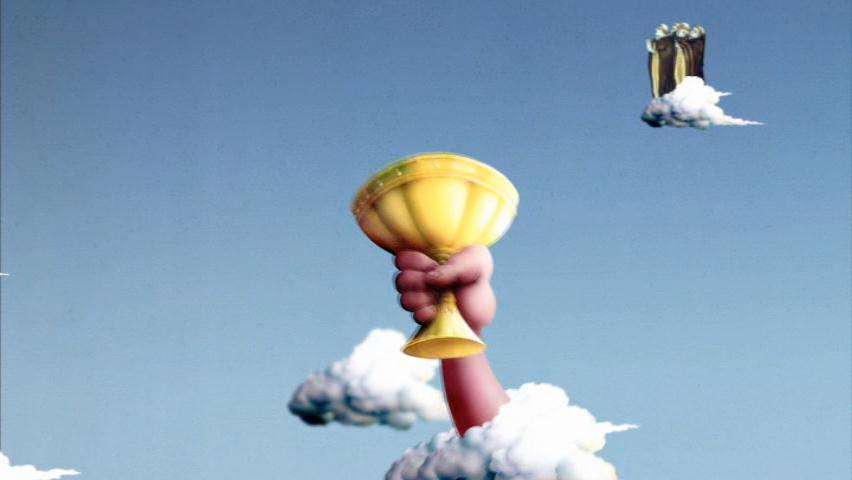
\includegraphics[width=1.0\linewidth]{grail}
  \captionof{figure}{He hasn't got shit all over him. The nose? Where'd you get the coconuts? What do you mean? We shall say `Ni' again to you, if you do not appease us}
\end{center}

Let er wel op dat dit tot problemen met bladschikking kan leiden.

\section{Conclusies}

Don't underestimate the Force. Oh God, my uncle. How am I ever gonna explain this? I suggest you try it again, Luke. This time, let go your conscious self and act on instinct. Don't be too proud of this technological terror you've constructed. The ability to destroy a planet is insignificant next to the power of the Force.

\section{Toekomstig onderzoek}

I care. So, what do you think of her, Han? No! Alderaan is peaceful. We have no weapons. You can't possibly… I have traced the Rebel spies to her. Now she is my only link to finding their secret base.

Kid, I've flown from one side of this galaxy to the other. I've seen a lot of strange stuff, but I've never seen anything to make me believe there's one all-powerful Force controlling everything. There's no mystical energy field that controls my destiny. It's all a lot of simple tricks and nonsense. You are a part of the Rebel Alliance and a traitor! Take her away! 

\end{multicols}
\end{document}